% ---------
%  Compile with "./build.sh"
% --------

\documentclass[10pt]{article}
\usepackage{amsmath}
\usepackage[margin=1in]{geometry}
\usepackage{import}
\usepackage{amssymb}
\usepackage{float}
\usepackage{listings}
\usepackage{graphicx}
\usepackage{cite}
\usepackage{subcaption}
\usepackage[ruled,vlined]{algorithm2e}
\usepackage[utf8]{inputenc}		% Allow some non-ASCII Unicode in source
\title{CS 581 Final Project: Improving the Scalability of Phylogenetic Placement Methods}
\author{Elizabeth Koning and Malachi Phillips}
\date{December 9, 2020}

\begin{document}

\vspace{-1cm}
\maketitle

\section{Introduction}

Phylogenetic placement is useful for tree construction and sequence classification. In the case of tree construction, phylogenetic placement can be a scalable way to construct a phylogeny. In the case of sequence classification, placement is useful as it can place sequences near closely related taxa even if the taxon of the sequence is not present in the tree. In both of these cases, it is key to have approaches that are both scalable and accurate.
The two leading methods for phylogenetic placement are pplacer and APPLES. pplacer \cite{matsen_pplacer_2010} is a highly accurate maximum likelihood phylogenetic placement method. Its limitation is that it does not scale to large trees. According to Balaban and coworkers,  pplacer frequently fails to run on trees with over 1000 leaves \cite{balaban_apples_2020}.
For the trees they tested with 5000 leaves, pplacer failed 449 times out of 1000. APPLES has been tested to run on trees up to 200,000 sequences. However, on the trees where both APPLES and pplacer successfully place sequences, pplacer is much more accurate than APPLES.
We propose two approaches that aim to provide the accuracy of pplacer alongside the scalability of APPLES. The first approach, pplacerDC, uses pplacer in a divide-and-conquer method. The second approach, pplacerAPPLES, first uses APPLES to identify a probable placement region, and then uses pplacer to find a more accurate placement within the region.

\section{Experimental Design}

% TODO: include the rest of the experimental design

% TODO: this must include how we calculate delta error

\subsection{Error Assessment}

We compared our approaches to both pplacer and APPLES in both their accuracy and runtime.
To calculate the error, we used the delta error, which is the same measurement that was used by
Balaban and coworkers in \cite{balaban_apples_2020}.
It compares the set of bipartions for the tree that includes the estimated placement using one of the four methods to the set of bipartions in the tree with the correct placement.

The delta error is defined as
\begin{align*}
\Delta e(P) = \vert B(T^*) \backslash B(P) \vert - \vert B(T^* \upharpoonright_{\mathcal L}) \backslash B(T)\vert,
\end{align*}
where $\mathcal L$ denotes the leafset, \(P\) denotes the tree after placement, $T^*$ denotes the true tree on $\mathcal L \cup \{q\}$, $T^* \upharpoonright_{\mathcal L}$ denotes the true tree restricted to $\mathcal L$, and $B(\cdot)$ denotes the bipartition set of a tree \cite{balaban_apples_2020}.

Similarly to the strategy used by Balaban and coworkers (\cite{balaban_apples_2020}), we used a leave-one-out strategy for the tests.
Out of the set of sequences in the tree, 200 sequences are selected as query sequences.
For each of the query sequences, the leave-one-out strategy starts with the true tree, \(T\), and removes the sequence from \(T\), creating \(T'\).
Then, the placement software adds that query to \(T'\) to obtain the estimated placement.

\subsection{Data}

For the data, we tested the methods on the RNASim-VS dataset from \cite{balaban_apples_2020}. This dataset is sampled from the larger RNASim dataset with varying numbers of sequences. It includes five replicates for 500, 1000, 5000, 10,000, 50,000, and 100,000 sequences, and one replicate for 200,000 sequences.

% We also used the 1000M1 data sets from \cite{sate} to examine model conditions where the rate of evolution varies. These datasets are for small, medium, and long gap lengths. Each set has 1000 sequences and 20 replicates. [NOTE: decide if we include this at all, but obviously we need to run it that way before we can include this info]

\subsection{Hardware}

We performed the analysis on NCSA's Blue Waters. Each Blue Waters XE node has 16 cores.

% TODO: actually make the results be from BW instead of Monza. Probably want to include more info about BW too

\section{Methods}

We developed two novel approaches and assess them in comparison to pplacer and APPLES.
Both of the methods accept input similar to that of pplacer and APPLES:
each requires a backbone tree that includes all sequences except the query sequence and a multiple sequence alignment (MSA) including all sequences and the query sequence.
The output is the backbone tree with the query sequence placed.
In addition, each requires the selection of the maximum size of the subtrees that are passed to pplacer, and the version using pplacer and APPLES requires the selection of the number of subtrees to assess using pplacer.

\subsection{pplacerDC}

The first method is a divide-and-conquer version of pplacer (pplacerDC).
The first step of the method is to decompose the backbone tree into subsets.
pplacerDC finds a centroid edge in the backbone tree that separates the leaf
sets into two with approximately equal size.
The decomposition is recursively applied to each subtree containing more
than the maximum allowable number of leaves.
The maximum size of the subtrees can be selected as a command line option, and should be small enough that pplacer can successfully place the query.
At the same time, however, 
pplacer reliably places on trees of 1000 sequences, but frequently failed for 5000 sequence trees \cite{balaban_apples_2020}.
The authors maintain that this was their own experience using pplacer, too.
If the maximum size is larger than the backbone tree, then running pplacerDC will be equivalent to running pplacer alone.

After dividing the tree into disjoint subsets, each step of the pplacerDC pipeline
is embarassingly parallel.
First, pplacerDC uses pplacer independently on each of the subtrees to determine tentative
query placements.
Each tentative query placement is then grafted onto the backbone tree, yielding a candidate
resultant tree and placement.
raxml-ng \cite{raxml} is then used in fixed tree topology, fixed branch length mode to evaluate
the log-likelihood of the resultant tree.
Each candidate placement position is scored using raxml-ng, and the placement position
with the largest log-likelihood score is returned by pplacerDC.
A schematic of the pipeline for pplacerDC is shown in fig \ref{fig:pplacerDC-pipeline}.
Pseudocode for pplacerDC is shown in alg \ref{alg:approach1}.
In order to be applicable in either a shared or distributed memory context,
two versions of pplacerDC are implemented in Python.
The first is tailored to running on shared memory machines using Python's
native thread pool paradigm.
The second, however, is written using the message passing interface (MPI) standard
bindings implemented in mpi4py and is tailored for distributed memory machines \cite{mpi4py-paper}.

\begin{figure}[h]
\centering
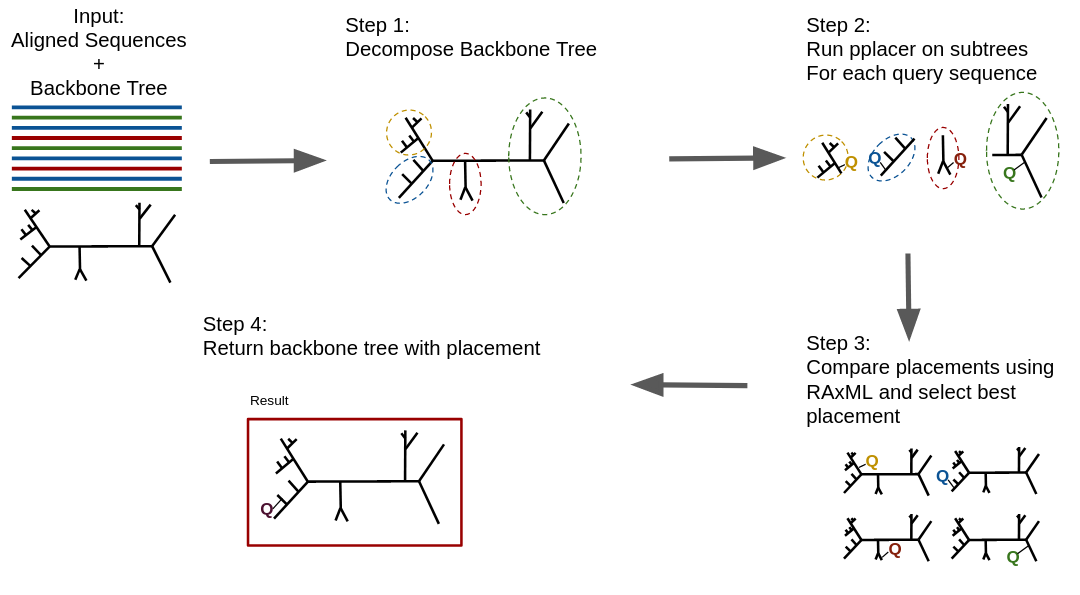
\includegraphics[width=\textwidth]{Figs/pplacerDCpipeline.png}
\caption{Pipeline for pplacerDC approach.}
\label{fig:pplacerDC-pipeline}
\end{figure}

\begin{algorithm}[h]
\SetKwFor{ParallelFor}{parallel for}{do}{endfor}
\SetAlgoLined
\KwResult{$T'$, tree T with query sequence $q$ added}
\KwIn{Tree $T$ on $N$ sequences, the MSA of $N+1$ sequences, and query sequence $q$}
 // $\operatorname{centroidDecomposition}$ decomposes a tree into roughly equal size, disjoint parts until the trees are no larger than the prescribed size.\;
 // $\operatorname{modifyTree}$ adds sequence to a tree based on the sequence's location in the a subtree with the sequence added\;
 $\{T_1,\dots,T_n\} \leftarrow \operatorname{centroidDecomposition}(T,1000)$\;
 $\{S_1, \dots, S_n\} \leftarrow 0$ // Score for each tree\;
 \ParallelFor{$i=1,\dots,n$}{
  // Place query sequence $q$ into the subtree\;
  $T'_i \leftarrow \operatorname{pplacer}(T_i, q)$\;
  // Add the location of the query sequence $q$ to a copy of $T$\;
  $T_{q_{i}} \leftarrow \operatorname{modifyTree}(T, T'_i, q)$\;
  // $\operatorname{RAxMLScorer}$ runs RAxML in fixed tree mode.\;
  // The output score is the maximum likelihood found on the tree.\;
  $S_i \leftarrow \operatorname{RAxMLScorer}( T_{q_{i}})$\;
 }
 // Do a maxLoc reduction for the tree\;
 $bestTreeIndex \leftarrow \operatorname{argmax}_{i} (S_1,\dots,S_n)$\;
 return $T'_{q_{bestTreeIndex}}$\;
 \caption{divide-and-conquer pplacer}
 \label{alg:approach1}
\end{algorithm}

\subsection{pplacerAPPLES}

The second method combines APPLES and pplacer, aiming to achieve the accuracy of pplacer with the scalability of APPLES.
First, the method runs APPLES with the query sequence and full backbone tree.
The method then samples a number of clades, sans the query leaf, with leafsets smaller
than a prescribed size.
The number of subtrees to use and the maximum size of the subtrees is selected through the command line.
As for pplacerDC, the maximum size of the subtree should be selected to be small enough to be handled by pplacer.
At the same time, however, considering a larger clade could yield a more accurate phylogenetic placement.
The method then uses pplacer to place the query sequence into each of the sampled clades, yielding
an ensemble of tentative placement positions, including the one from APPLES.
Finally, the method uses raxml-ng in fixed tree topology, fixed branch length mode to evaluate
the log-likelihood score for the backbone tree with a given placement.
Each tentative placemenet, including the one generated by APPLES, is compared.
The placement maximizing the log-likelihood score is the tree returned by pplacerAPPLES.
A schematic of the pipeline for pplacerDC is shown in fig \ref{fig:pplacerAPPLES-pipeline}.
Pseudocode for pplacerDC is shown in alg \ref{alg:approach2}.

\begin{figure}[h]
\centering
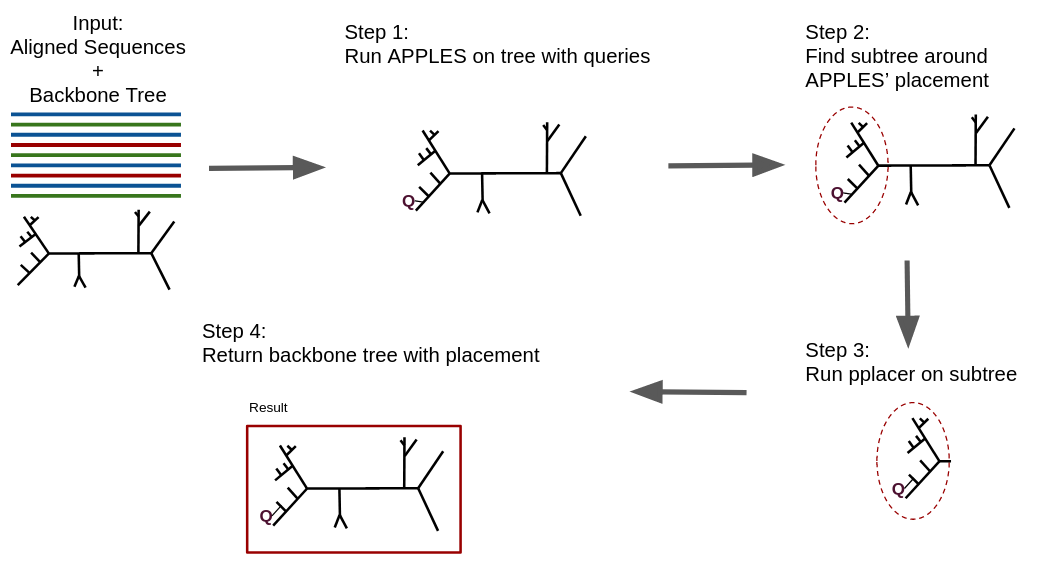
\includegraphics[width=\textwidth]{Figs/pplacerAPPLESpipeline.png}
\label{fig:pplacerAPPLES-pipeline}
\caption{Pipeline for pplacerAPPLES approach
}
\end{figure}

\begin{algorithm}[h]
\SetKwFor{ParallelFor}{parallel for}{do}{endfor}
\SetAlgoLined
\KwResult{$T'$, tree T with query sequence $q$ added}
\KwIn{Tree $T$ on $N$ sequences, the MSA of $N+1$ sequences, query sequence $q$,
and the number of clades considered, $N_{clades}$.
}
 // $\operatorname{modifyTree}$ adds sequence to a tree based on the sequence's location in the a subtree with the sequence added\;
 // $\operatorname{getRegion}$ finds a subtree containing the sequence with a maximum number of sequences\;
  // Run APPLES\;
  $T'_{APPLES} \leftarrow \operatorname{APPLES}(T, q)$\;
  // It could be the case that APPLES produces the best score\;
  $S_{apples} \leftarrow \operatorname{RAxMLScorer}( T'_{apples})$\;
  $\{S_1, \dots, S_{N_{clades}}\} \leftarrow 0$ // Score for each clade\;
  \ParallelFor{$i=1,\dots, N_{clades}$}{
    // Identify (random) region of T where q was placed with fewer than 1000 sequences\;
    $T_{i} \leftarrow \operatorname{getRegion}(T'_{APPLES}, q, 1000)$\;
    // Run pplacer on the area of T around the placement of q\;
    $T'_{pplacer} \leftarrow \operatorname{pplacer}(T_{i})$\;
  // Add the location of the query sequence $q$ to a copy of $T$\;
  $T_{q_{i}} \leftarrow \operatorname{modifyTree}(T, T_{i}, q)$\;
  // $\operatorname{RAxMLScorer}$ runs RAxML in fixed tree mode.\;
  // The output score is the maximum likelihood found on the tree.\;
  $S_i \leftarrow \operatorname{RAxMLScorer}( T_{q_{i}})$\;
  }
 // Do a maxLoc reduction for the tree\;
 $bestTreeIndex \leftarrow \operatorname{argmax}_{i} (S_{apples},S_1,\dots,S_n)$\;
 return $T'_{q_{bestTreeIndex}}$\;
\caption{APPLES with pplacer}
 \label{alg:approach2}
\end{algorithm}

\section{Results}

Delta error results for the RNASim-VS data sets
are shown below in figures \ref{fig:error500,fig:error1000,fig:error5000,fig:error10000}.
\begin{figure}[h]
\begin{subfigure}{0.5\textwidth}
\centering
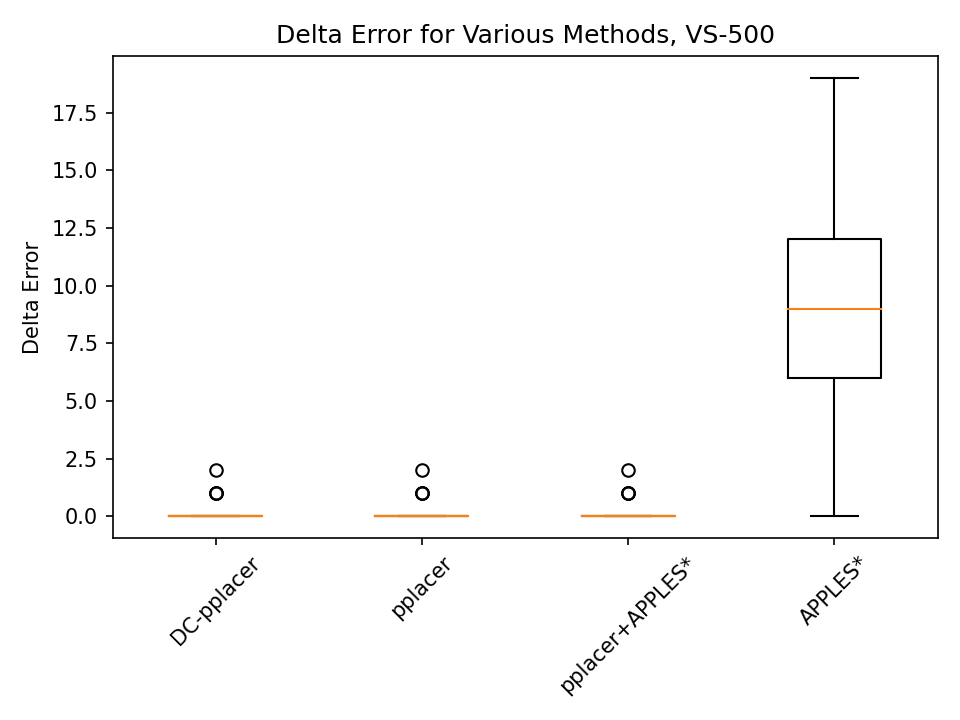
\includegraphics[width=\textwidth]{Figs/VS-delta-error-500.png}
\caption{Delta Error for RNASim-VS with 500 sequences}
\label{fig:error500}
\end{subfigure}
\begin{subfigure}{0.5\textwidth}
\centering
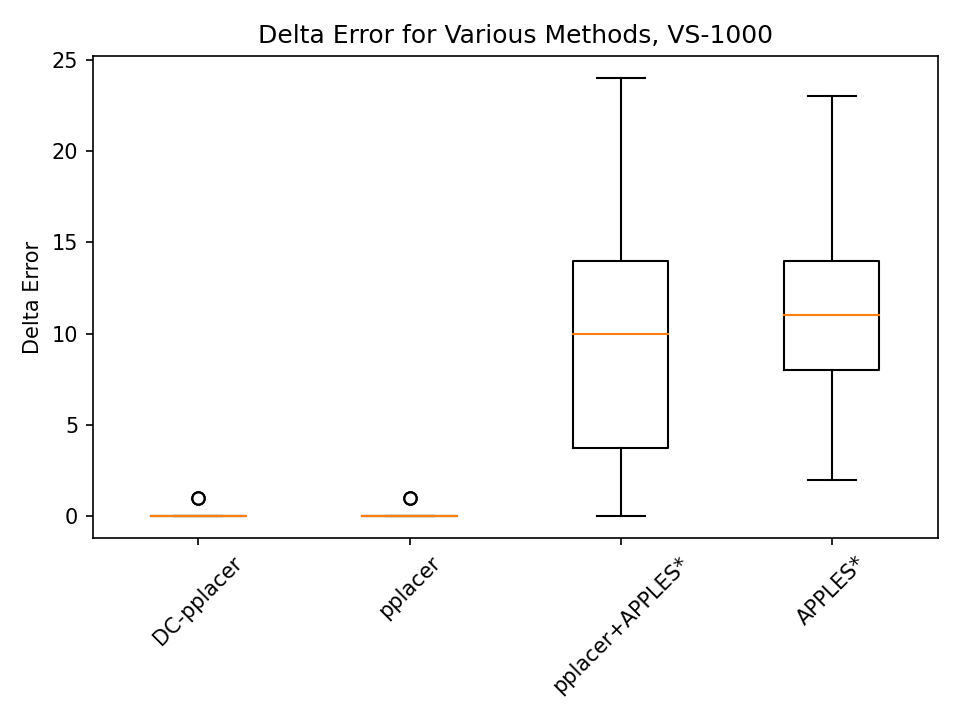
\includegraphics[width=\textwidth]{Figs/VS-delta-error-1000.png}
\caption{Delta Error for RNASim-VS with 1000 sequences}
\label{fig:error1000}
\end{subfigure}\\
\begin{subfigure}{0.5\textwidth}
\centering
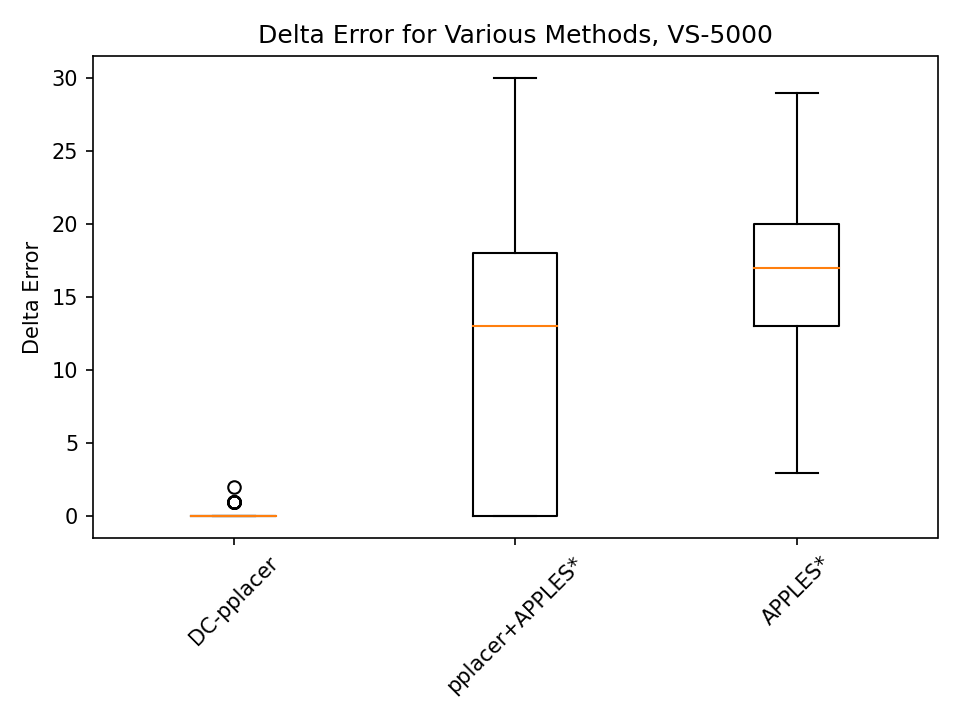
\includegraphics[width=\textwidth]{Figs/VS-delta-error-5000.png}
\caption{Delta Error for RNASim-VS with 5000 sequences}
\label{fig:error5000}
\end{subfigure}
\begin{subfigure}{0.5\textwidth}
\centering
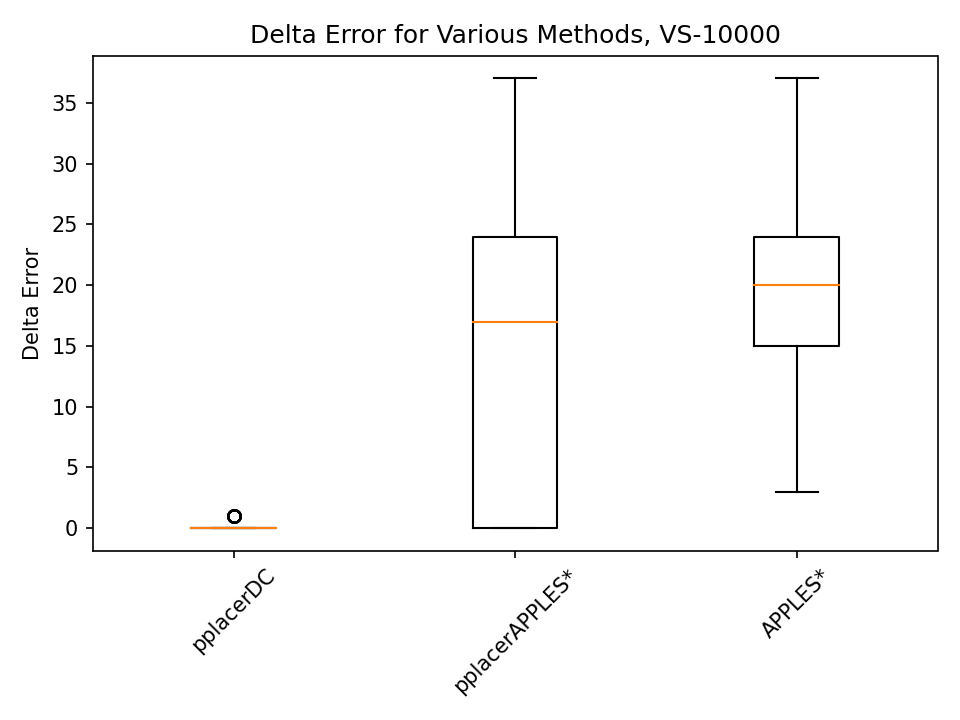
\includegraphics[width=\textwidth]{Figs/VS-delta-error-10000.png}
\label{fig:error10000}
\caption{Delta Error for RNASim-VS with 10,000 sequences}
\end{subfigure}\\
\begin{subfigure}{0.5\textwidth}
\centering
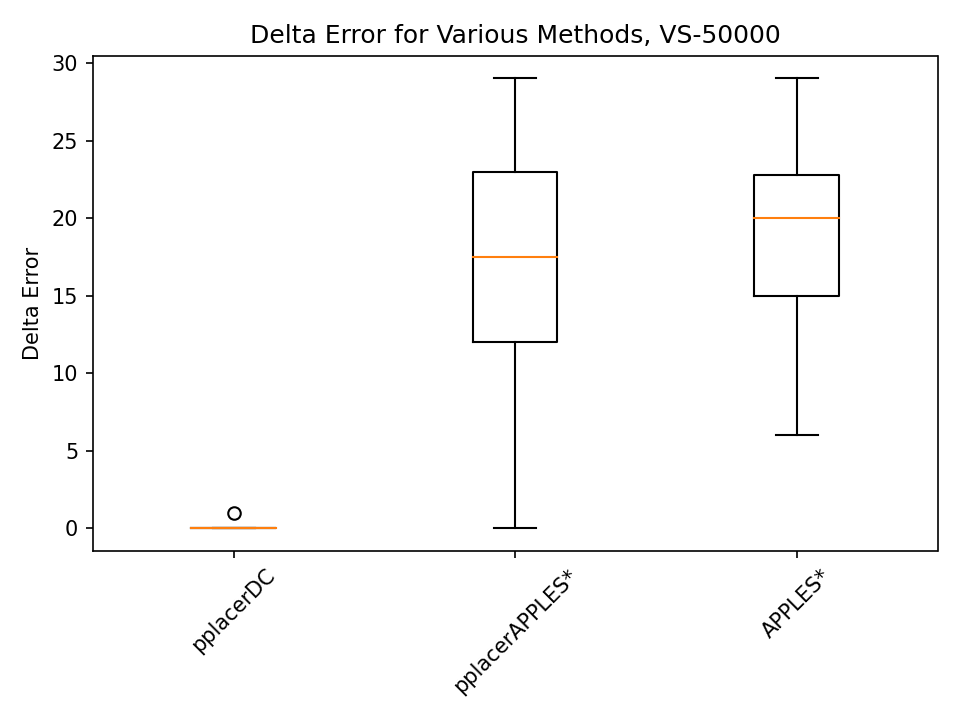
\includegraphics[width=\textwidth]{Figs/VS-delta-error-50000.png}
\caption{Delta Error for RNASim-VS with 50,000 sequences}
\label{fig:error50000}
\end{subfigure}
\end{figure}

In order to observe the effect of subproblem size and accuracy for pplacerDC,
the maximum subproblem size is varied on the RNASim-VS-5000 leaf data set.
Three of the 5 replicates with 100 query species per replicate are
considered for 100, 500, and 1000 leaf subproblems.
The results are shown in fig \ref{fig:varying-size}.
As shown in the figure, the choice of sub problem size does not seem
to have an effect on the error observed.
This is an important consideration with respect to parallel computing,
since allowing a smaller subproblem size allows
for increased parallelism in running pplacerDC.
\begin{figure}[h]
\centering
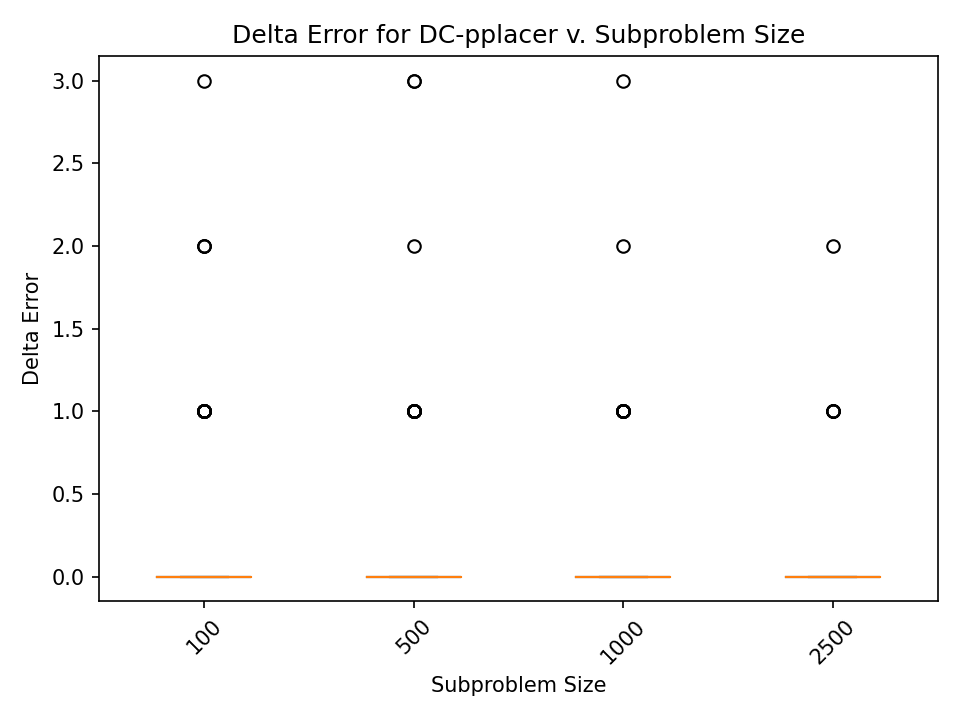
\includegraphics[width=\textwidth]{Figs/varying-subproblem-size.png}
\caption{Effect of changing the maximum pplacer size on the error for DCpplacer.}
\label{fig:varying-size}
\end{figure}
Runtime results on 12 threads on Monza are shown below in figure \ref{fig:timing-results}.
A maximum of 2,500 taxa are considered for the pplacerDC decomposition and the clade
sampling for pplacerAPPLES.
For the latter method, only a single clade is sampled.
\begin{figure}[h]
\centering
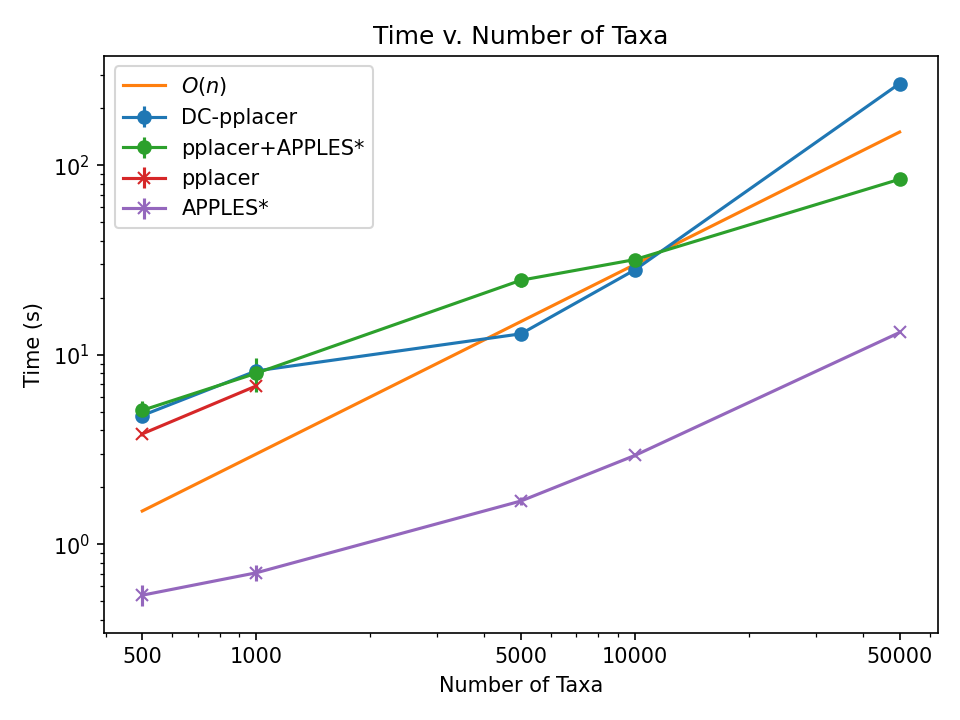
\includegraphics[width=\textwidth]{Figs/VS-timing-results.png}
\caption{Runtime on Monza for 12 threads. Time is average time required to place a single query sequence.}
\label{fig:timing-results}
\end{figure}

% TODO: update all figures to use Blue Waters results

% TODO: include discussion of all results


Through the experiments, we found that pplacerDC was significantly more accurate than APPLES for the datasets we tested on.

% TODO: expand this section a lot

\section{Discussion}

% TODO: write this section

\section{Conclusions}

While the code is not currently open-sourced and freely available, a version of the code
may be accessed with details in the appendix.
The authors intend to make the code open-source and freely available shortly.

\bibliographystyle{ieee}
\bibliography{cs581-project}

\end{document}
